\documentclass{beamer}
\usepackage{multirow}

\usepackage[T1]{fontenc}
\usepackage{amsmath}
\usepackage{MnSymbol}
\usepackage{IEEEtrantools}
\usepackage{hyperref}
\usepackage{url}
\usepackage{amsmath,stackengine}
\stackMath
\usepackage{natbib}
\nocite{*}
\usetheme{Madrid}
\title{Contagion Effect Estimate Through the Lens of Different Statistical Methods}
\author{Brisilda Ndreka\\
Department of Statistics\\
University of Connecticut
} 
\date{ December 5, 2022}

\begin{document}
\maketitle 
%=================================================
\begin{frame}
\frametitle{Outline}
\begin{itemize}
   \item  Influence (behaviour) model  using dynamic linear model 
     \vspace{10pt}
    \item Why is estimating contagion effect in social science considered a challenged  process?
    \vspace{10pt}
    \item Alternative methods which help to achieve a better estimation of the true contagion effects
    \vspace{10pt}
    \item  Defining the estimation method that has the  best performance
\end{itemize}
\end{frame}
%=================================================
\begin{frame}
\frametitle{Background}
\begin{itemize}
    \item Contagion effect, also referred as social influence effect or peer effect, is the tendency of a person or group of individuals to follow the behaviour of some reference group that they participate in.
    \vspace{10pt}
    \item The dynamic liner model used to estimate social influence effect is referred to as behaviour model \cite{XU2018101}, \cite{article}
 \[  Y_{it}=\beta_{0}+\beta_{\stackengine{2pt}
  {\scriptstyle 1}
  {\scriptstyle\text{Lagged Dependent Variable}\rule[3pt]{2ex}{.5pt}\mkern-5mu\raisebox{1.3pt}
  {\stackon[-.1pt]{\rule{.5pt}{9.1pt}}{\uparrow}}}{U}{r}{F}{T}{S}}Y_{i t-1}+\beta_{\stackengine{2pt}
  {\scriptstyle 2}
  {\scriptstyle\raisebox{1.1pt}{\stackon[-.1pt]{\rule{.5pt}{9.1pt}}{\uparrow}}
  \mkern-5mu\rule[1pt]{2ex}{.5pt}\text{Contagion Effect}}{U}{l}{F}{T}{S}}
 \frac{\Sigma Z_{ij t-1}Y_{j t-1}}{\Sigma Z_{ijt-1}}+ \beta_{3}X_{it-1}+\beta_{4}C_{i}+\epsilon_{it}.
 \]   
 $Y$ is the behavior outcome of interest, $X$ is the covariates that may affect behavioral outcome $Y$, $Z$ is network and $C$ is the time-invariant unobserved trait.  
\end{itemize}
\end{frame}
%=================================================
\begin{frame}
\frametitle{Why it is Difficult to Identify Social Influence Effect (Contagion Effect)? }
\begin{itemize}
\item Consider the example: In daily life, friends in social networks exhibit similar personality  and behaviors. Why doe this phenomena happen? \\
Answering this questions can result in two directions of thinking:
\vspace{10 pt}
\begin{itemize}
\item Social influence effect: Individuals can influence their friends behaviour, or transform their friends characteristics to be similar to theirs. 
\vspace{10pt}
\item Homophily: In which people with similar characteristics or behaviors are more likely to be friends. 
\end{itemize}
\vspace{10 pt}
\item Consequently, homophily has been identified as a major confounding factor to estimate the influence in social network effect. 

\end{itemize}
\end{frame}
%=================================================
\begin{frame}
\frametitle{This Challenge Can be Treated  as  a Function of an Omitted Variable Bias}
\begin{itemize}
\item{Separating homophily from  social influence is
a challenging process, particularly when the influence effect  is confounded with latent homophily caused by unobserved trait.}
\vspace{10pt}
\begin{itemize}
    \item If an unobserved variable affects behavioral model and selection process, this cause estimation problems of the social influence effect \cite{XU2018101}. Alcohol behaviour among teenager example.
    \begin{figure}[h!]
  \centering
  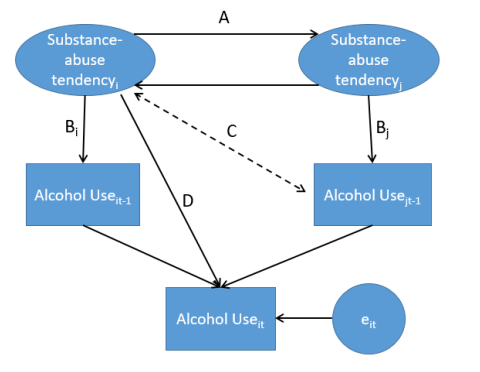
\includegraphics[width=.4\linewidth]{rx.png}
  \caption{Omitted variable bias/  (Xu, 2021)}
  \label{fig:fig1}
\end{figure}
\end{itemize}
\end{itemize}
\end{frame}
%=================================================
\begin{frame}
\frametitle{Methods Used to Estimate Latent Variable }
\begin{itemize}
\item Considering existence of biases of the contagion effects if omitted variables in the influence/selection process exist, four estimation methods are applied to estimate this latent trait: 
\vspace{10pt}
\begin{enumerate}
 \item \textbf{Latent Space Adjusted Method}  \textit{\cite{XU2018101}}.
\vspace{10pt}
\item \textbf{SDNE: Structural Deep Network Embedding}\textit{\cite{wang2016structural}}.
\vspace {10pt}
\item \textbf{Node2Vec} \textit{\cite{DBLP:journals/corr/GroverL16}}
\vspace {10pt}
\item \textbf{Latent Factor Model} \textit{\cite{minhas2019inferential}}
\end{enumerate}
\vspace {10pt}
\item Furthermore, fixed  effect estimator are used  as baseline comparisons. The objective of the study is to determine the method that has the best performance and help to reduce bias of estimating peer effect.
\end{itemize}
\end{frame}
%================================================
\begin{frame}
\frametitle{ 1: Latent Space Adjusted Approac}
\begin{itemize}
\item Assume the existence of an unobserved trait that co-determines influence and selection process
\vspace{10pt}
\item  It is based on latent space  model set up \cite{hoff2002latent} to derive "latent social positing" 
\begin{figure}[h!]
  \centering
  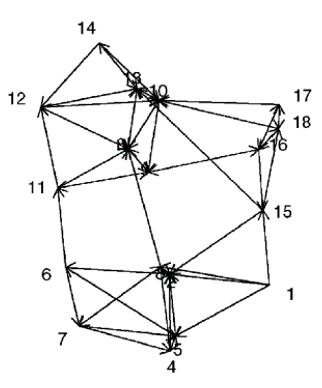
\includegraphics[width=.25\linewidth]{pff.png}
  \caption{Latent Space Estimates / (Hoff et al, 2016)}
  \label{fig:fig1}
\end{figure}
\item Adjust for the dynamic models: use latent position for all available time points as proxies for the unobserved trait
\end{itemize}
\end{frame}
%================================================
\begin{frame}
\frametitle{2: SDNE }
\begin{itemize}
\item  SDNE is machine learning algorithm  with the goal of turning a graph into a computationally  absorbable format. 
\vspace{10pt}
\item  Network embedding intends to capture and carry out the network structure of a network structure by using low-dimensional representations of vertexes in networks. 
\vspace{10pt}
  \item   It is  a method that is
able to effectively capture the highly non-linear network structure.
\end{itemize}


\end{frame}
%=================================================

\begin{frame}
\frametitle{3: Node2vec}
\begin{itemize}
\item  Node2vec is a random walk based method, which  use a walk approach to generate (sample) network neighborhoods for nodes is a random walk based method which  uses a walk approach to generate (sample) network neighborhoods for nodes. 
\vspace{10 pt}
\item Algorithm computes a vector representation of a node based on random walks in the graph.
\vspace{10 pt}
\item  Two parameters control the probability of moving in the graph;
\begin{itemize}
\item return hyperparameter, p 
\item inout hyperparameter, q 
\begin{figure}[h!]
  \centering
  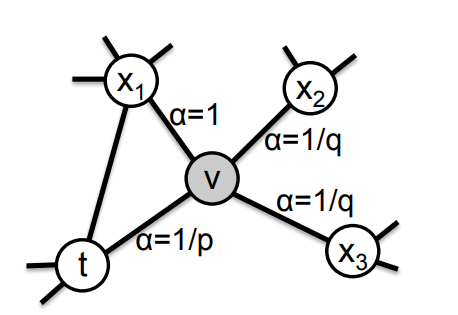
\includegraphics[width=.4\linewidth]{n2v.png}
  \caption{Random walk procedure in node2vec/ (Grover et al, 2016)}
  \label{fig:fig1}
\end{figure}
\end{itemize}

\end{itemize}
\end{frame}
%=================================================

\begin{frame}
\frametitle{4: Latent Factor Model}
\begin{itemize}
\item Each node $i$ has an unknown latent factor $c_{i}\in R^{k}$
\vspace{10pt}
\item The probability of the nodes $i$  and $j$ to form a tie depends on their latent factors
 \[P(Z_{ij}=1|c_{i},c_{j})=\alpha+ c_{i}^{T} \Lambda c_{j}
    \label{3},\]  $\Lambda$ a$ K\times K$ diagonal matrix.
\vspace{10pt}
\item  Multiplicative effects, capture higher-order dependence patterns  after accounting for any known covariate information.

\end{itemize}
\end{frame}
%=================================================
\begin{frame}
\frametitle{Simulation Setting}
\begin{itemize}
\item Four estimation methods are considered  and each of them estimate latent variable using  dimensions of 1 and 3.
\vspace{10pt}
\item Statistical software packages to accomplish the analysis for each presented methods:
\begin{itemize}
\item  latent-space adjusted : \textit{ergm} package withR  \textit{\cite{your-key-here}}
\vspace{5pt}
\item latent-factor: \textit{AMEN} with R  \textit{\cite{https://doi.org/10.48550/arxiv.1506.08237}}
\vspace{5pt}
\item Node2vec: \textit{node2vec}, python3 \textit{\cite{DBLP:journals/corr/GroverL16}}
\vspace{5pt}
\item SDNE: \textit{EasyGraph0.2} with Python 
\href{https://easygraph.github.io/docs/reference/graph_embedding.html}{source information can  be found here}
\end{itemize}

\vspace{10pt}
\item{Networks studied, small networks with 40 nodes and  with 80 nodes, number of time points  $T=2$ and $5$}
\end{itemize}
\end{frame}
%=================================================
\begin{frame}
\begin{itemize}
\item{The real value of the peer influence effect and lagged dependent variable, are considered when of $\beta_{1}, \beta_{2} \in \{ 0.1, 0.4, 0.7\}$ }
\vspace{10pt}
\item Level of homophily based on the unobserved trait considered relatively high with $\alpha_{2}=0.4$.
\vspace{10pt}
\item{After estimating latent trait $C$, use it as proxy in the influence model to define contagion effect}
\begin{itemize}
    \item  Influlence moddel: \[  Y_{it}=\beta_{0}+\beta_{1}Y_{i t-1}+\beta_{2} \frac{\Sigma Z_{ij t-1}Y_{j t-1}}{\Sigma Z_{ijt-1}}+ \beta_{3}X_{it-1}+\beta_{4}C_{i}+\epsilon_{it}.\] 

\item{Social networks were generated using  selection model:}
 \[ P(Z_{ij}=1|c_{i},c_{j},x_{ij},\alpha, \beta)= \Phi(\alpha+\alpha_{1}|X_{i}-X_{j}|-\alpha_{2}|C_{i}-C_{j}|)
    \label{eq.4}\]
 
\end{itemize}
   \item The metric used to compare methods’ performances is the peer effect and lagged dependent variable bias. 
\end{itemize}
\end{frame}
%=================================================
\begin{frame}
\frametitle{Simulation Results: Contagion Effect }
\begin{figure}[H]
  \centering
  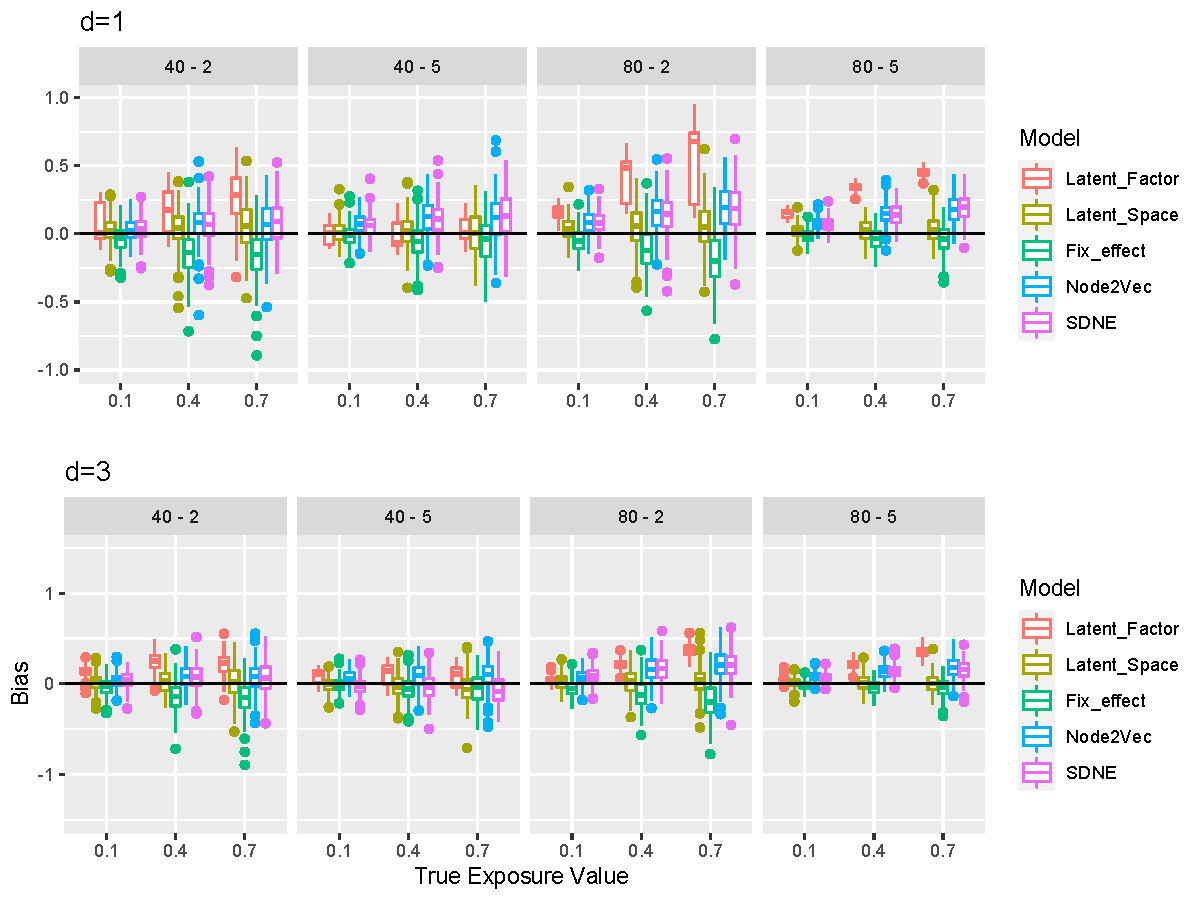
\includegraphics[width=10 cm, height=7cm ]{plot1.pdf}
  \caption{ Bias Distribution for Contagion Effect}
  \label{Fig:fig1}
\end{figure}
\end{frame}
%=================================================
\begin{frame}
\frametitle{ Results Interpretation}
\begin{itemize}
\item  The magnitude of bias is smaller for
all estimation methods when we include more time points (T =5 bias estimate smaller than T=2).
\vspace{10pt}
\item Latent space estimates bets-perform compare to other methods in terms of estimating contagion effects, as it leads to the smallest bias.
\vspace{10pt}
\item Overall, Node2Vec estimates have small
bias, but performance is  better when peer effect and network size is small. Moving to larger network method decreases the performance. 
\vspace{10pt}
\item Latent factor estimates are more unstable,
as they have  higher bias mostly for small dimension and small time points. Performance improved when these two factors increased.
\end{itemize}
\end{frame}
%=================================================
\begin{frame}
\frametitle{ }
\begin{itemize}

\item SDNE archived good results when network size was relatively small (almost the same bias estimation as latent space), but lost the efficiency in large networks. 
\vspace{10pt}
\item Fixed effects estimates produce the
biggest bias among all estimators.
\vspace{10pt}
\item We should point out that  the latent space and latent factor model require a large computing time, since both methods use MCMC (Marcov Chain Monte Carlo Algorithm) in the estimation process.
\end{itemize}
\end{frame}

%=================================================
\begin{frame}
\frametitle{Simulation Results: Lagged Dependent Variable Bias.  }
\begin{figure}[H]
  \centering
  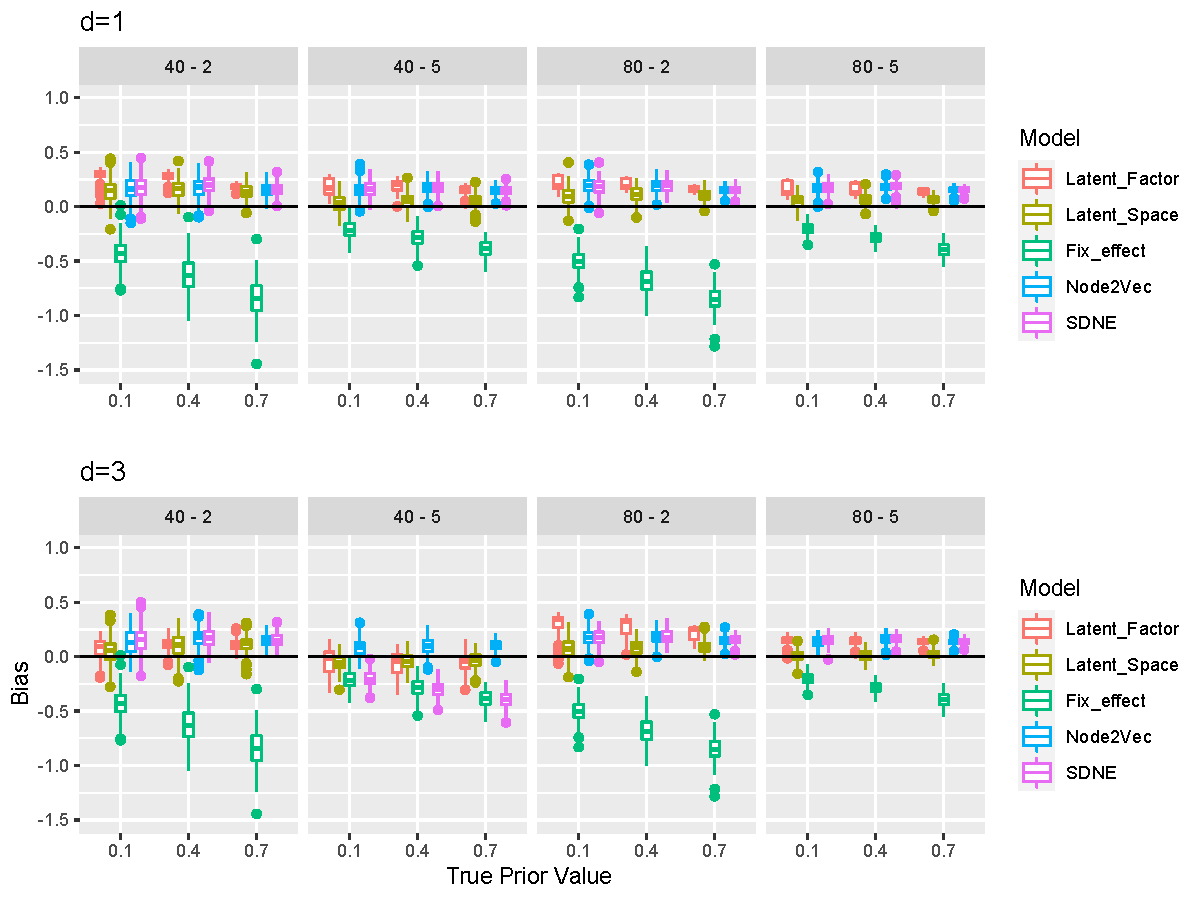
\includegraphics[width=10cm, height=7cm]{plot2.pdf}
  \caption{Bias Distribution for Coefficient of Lagged Dependent Variable}
  \label{Fig:fig2}
\end{figure}
\end{frame}

%=================================================
\begin{frame}
\frametitle{Results Interpretation: }
\begin{itemize}
\item Latent space adjusted approach produces much smaller bias in estimating the lagged independent variable  (previous behaviour) compared to other methods.
\vspace{10pt}
\item As in the contagion effect the bias  value is smaller for all estimation methods when we include more time points (compare for T=2 \& T=5).
\vspace{10pt}

\item Latent factor estimates show small bias when the true coefficient large , but is unstable for other scenarios.
\vspace{10pt}
\item Fixed effects estimates are always negatively biased and unfavorable in dynamic netwrok analysis.
\vspace{10pt}
\item In general Node2vec estimates  produce a small bias in contradiction to SDNE that was more efficient with contagion estimate. 
\end{itemize}
\end{frame}
%=================================================
\begin{frame} [allowframebreaks]{Reference}
%\printbibliography
\small\bibliography{ref}
\bibliographystyle{plainnat}
\end{frame}
\end{document}
%=================================================
